

\chapter{SVR+Q+MCKP分块逼近模型在广告预算分配中的研究}

% 首先介绍多渠道广告投放资金分配问题使用强化学习研究的现状(没有利用强化学习解决该问题的文献,存在的主要问题:数据量较少,导致值函数估计不准确等问题,收敛速度慢,说明本文采用非参数化建模的原因,非参数化建模又存在什么问题,针对此问题又是如何解决的)
% 介绍深度强化学习
% 介绍本文提出的混合网络模型算法
% “我知道我的广告费有一半浪费了,可是我不知道浪费的是哪一半。”美国费城商人约翰·华纳梅克的这句自嘲式的调侃简直让人抓狂——似乎你绞尽脑汁想出的营销点子就是为了达到一个目的——尽量让广告费被浪费得少一点而已。

\section{直复营销下广告预算分配问题阐述}
这一节,首先介绍了在直复营销体系下,基于第三方广告代理商进行广告投放的应用场景及其具体的投放过程。然后,说明了多渠道广告投放的目标是追求全渠道的LTV最大化,以此作为选择强化学习解决该问题的依据。最后,介绍了在广告投放预算分配场景中所面临的三个特点,并针对这些特点进行分析,提出对应的解决思路,来作为本章研究的出发点。

\subsection{广告预算分配场景}
美国直复营销协会(American Direct Marketing Association,ADMA)\footnote{http://www.the-dma.org/}将直复营销(Direct Response Marketing)定义为一种市场营销体系,运用一种或几种广告媒介在任何地点产生可以度量的反应或交易。直效营销仅仅属于直复营销中的一种应用场景,它特指不通过第三方,中间人,而直接对客户进行推广和营销,以维持企业与客户的良好关系。但是,在此场景下需要企业有充足的客户资源和大量的相关客户资料,这对于大部分企业是很难办到的,因为它需要很长时间的积累,特别是在日益激烈的市场竞争环境中,时间就是企业的生命。于是,为了快速获取用户、推广相关产品、扩大公司的收入,越来越多的企业选择通过第三方广告代理商(ad-agency)进行广告投放。

广告代理商除了帮助企业进行广告设计与策划以外,还有一部分更重要的工作,就是帮助广告主安排或代为购买媒介空间或时间。近年来,随着广告市场的不断发展和扩大,为了方便广告主高效的进行广告投放,大部分在线的广告代理商都建设了自己的广告投放平台,其投放流程如图
% $\ref{fig:ad_process}$
所示:在广告投放平台上,广告代理商(ad-agency)有很多可供选择的广告渠道(channel)资源,广告主在每次进行广告投放时需要提供一个广告投放策略,策略的内容包括在哪些渠道上投放广告以及对应投放多少金额的广告费。然后,广告代理商会按照广告主提供的投放策略,将相应的广告投放量通过各渠道投放给潜在顾客(广告的受众)。在广告投放结束后,广告代理商会将此次广告投放的直观效果反馈给广告主,同时广告主也可以通过追踪已经产生交易的顾客的后续信息,综合评价此次的投放效果。



通过以上的介绍,可以看到,在通过广告代理商投放广告的过程中,顾客可以及时接收到广告主发布的广告信息,而广告主也会收到响应顾客的响应反馈,因此广告主与顾客之间是存在互动性的。另外,广告主还可以根据广告代理商反馈的投放效果信息以及追踪用户未来的交易等方式去量化此次广告投放对企业的价值,因此效果是可衡量性的,所以,利用广告代理商进行广告投放的方式也属于直复营销体系的研究范围内。

在企业进行广告投放的真实业务中,为了保证财务帐面的稳定以及公司合理健康的发展,公司财务每个月都会提前给出该月的广告投放资金的预算,然后广告投放部门会在此预算下进行广告预算的合理分配,以使得公司的业务不断扩大、收入持续增长。但是,因为广告投放场景比较复杂,单纯靠广告投放人员制定预算分配策略往往很持续难达到好的效果,所以需要充分利用机器学习技术协助进行决策。

\subsection{基于全渠道的LTV值}
通常情况下,企业在进行广告投放时,为了能够更好的评价广告渠道的质量,而且为了能达到持久有效的营销效果,一般都会选择一个广告代理商进行为期一年或几年的持续投放。因此,广告投放是一个序列化的过程。

评价广告投放渠道质量的重要指标是该渠道的投资回报比(Return On Investment, ROI),即一定周期内,广告主通过广告投
放收回的价值占广告投入的百分比,计算方法如式\eqref{seq:roi}所示,其中Income表示收入额,Cost表示成本额,Investment表示投资额,一般情况下认为Cost和Investment是同一概念。
\begin{equation}\label{seq:roi}
\begin{aligned}
 ROI=\frac{Income-Cost}{Investment} \times 100\%
\end{aligned}
\end{equation}

然而,在广告投放的过程中,用户的反馈存在一定的延迟,而且某一时刻投放的广告会对后面时刻的广告投放效果产生一定程度的影响,所以不能仅仅使用即时的ROI值作为渠道质量的评价指标。比如,一个顾客在某一时刻看到某广告,但是并没有立刻产生正向反馈或者交易,而是在经过若干时间后的某一时刻才有正向反馈。那么,此时所产生的收益不单单与现在这个时刻的广告投放效果有关,还与之前的广告投放效果有关。所以,在计算广告投放所产生的回报时,应该要有全局观念。因此,在实际应用中,广告主一般将基于渠道LTV的ROI值作为选择广告渠道的指标,LTV是指渠道所产生的累积收益,只要将公式\eqref{seq:roi}中的Income换成渠道的LTV值即可。

考虑到企业进行广告投放的主要目的是为了尽可能的增加自身利润,如果单单只考虑渠道的ROI值,并不能得到对企业来说价值最大的投放策略。因为即使一个投放产生的ROI值很大,但是如果产生这个很大ROI值的那个投放花费很小的话,其利润不可能很大,这并不是企业所期望得到的最终效果。所以本章研究的给定预算下的广告投放资金分配问题,并不以ROI值作为评价指标,而是关注什么样的投放策略可以使企业产生的收益最大化,即广告渠道的LTV值最大化。

通过第二章的介绍,我们知道,强化学习在处理序列问题时,因为考虑到了延迟奖赏的问题,并且以追求累积奖赏最大化作为优化目标,所以将强化学习技术应用在广告投放领域,可以充分发挥其优势。

\subsection{广告预算分配特点}
% 多渠道/总预算限制/数据量少
解决好广告投放的资金预算分配问题,虽然有着很高的现实意义和商业价值,但是目前并没有引起很多学者和专家的注意。其中,最主要的原因就是没有在此领域公开的数据集。本文的数据是基于国内某公司在进行广告投放过程中所产生的真实数据,所以研究内容具有的实用性和真实性。

即便拥有了相关的广告投放数据,但是因为该领域还存在诸如场景复杂、数据量较少、固定预算约束等问题,不能直接将强化学习算法应用在该场景中。所以,本章从这些存在的问题作为出发点,结合强化学习进行分析,并提出了相应的解决方法。

对于大部分企业来说,广告投放是以天为单位进行的,所以投放数据量比较少,影响了模型的训练和学习,因此,为了提高数据的使用率,在强化学习模型中我们考虑使用非参数化函数逼近的方法进行Q值函数的学习。另外,通常情况下,为了达到全方位的效果,在进行广告投放时会选择多个渠道同时进行投放,因此,我们不能只考虑渠道自身的延迟反馈影响,而且还应该考虑渠道间的相互影响。最后,每一次的广告投放策略都需要在给定的固定预算约束进行,所以,我们在使用强化学习进行Q值估计之后,还要考虑如何进行合理的分配方法。

\section{SVR+Q+MCKP模型}
为了解决多渠道广告预算的资金分配问题,在我们的模型中,首先需要使用强化学习算法估算出当前时刻每一个渠道在每一种花费下可能产生的累积利润(即Q值),然后,再利用多选择背包问题(Multiple-Choice Knapsack Problem, MCKP)选择出每个渠道最合适的花费以使的企业产生的利润最大化。

然而,在真实的广告投放场景中,广告主进行广告投放的周期是相对较长的(一天一次),所能得到的数据也就相对较少。所以,在进行Q值函数逼近值时,要求我们高效的利用仅有的训练样本。然而,通过第二章的介绍,我们知道在参数化函数逼近方法中,线性逼近值函数的逼近能力较弱、效率较低,非线性函数(神经网络)逼近又需要有充足的训练样本。所以,综合考虑,我们选择了基于非参数化函数逼近的模型,因为该模型是一种基于样本的学习方法,具有较高的灵活性,而且适用于小样本数据。

但是,非参数化函数逼近常常存在着收敛性难移保证的问题。于是,本章提出了基于SVR+Q的分块强化学习模型,在该模型中,将对Q值函数逼近问题转化为高维特征空间中的线性回归问题,从而可以加快函数的收敛速度。另外,为了在小数据集下提高函数逼近的精度,提出分块逼近的思想,每个离散的行为作为一块,分别使用SVR+Q模型进行训练,最后再利用训练好的分块模型多路逼近Q值函数。在训练结束后,再使用MCKP问题解决资金的合理分配问题。

\subsection{问题的形式化定义}
下面给出多渠道广告投放预算分配问题的形式化描述:

假定在多渠道广告投放中给定的固定预算金额为$B$,广告投放的策略$\bm{x}=(x_{1},x_{2},\cdots,x_{n})$,即$x_{i}$是在第$i$个渠道上分配的投放金额,$n$为渠道的数量。令$R(\bm{x})$是在给定预算分配策略$\bm{x}$下的累积利润。所以,我们可以将问题形式化描述为:
\begin{equation}\label{seq_ad_goal}
\begin{split}
&max_{\bm{x}} R(\bm{x}),\\
&s.t. \sum_{i=1}^{n} x_{i} \leqslant B \text{且} x_{i} \geq 0.
\end{split}
\end{equation}

也就是说,我们的目标是将预算金额$B$在$n$个渠道上进行合理划分,以使得整体收益最大化。但是,在进行划分前,我们需要清楚的知道当前时刻每一个渠道在每一种可能的花费下会产生什么样的价值(累积利润)。这里,我们采用的是基于SVR+Q多路分块逼近强化学习模型。

\subsection{分块多路逼近思想}
经过前面的分析,我们知道,在广告投放场景中,可获得的数据量比较少,如果将所有渠道合在一起进行建模,很难拟合出可靠的值函数变化规律。所以,我们采取分渠道进行建模的思路。进一步地,每个渠道在进行值函数的逼近时,考虑到状态空间和行为空间(广告花费)是连续的,因为数据样本较少也会造成状态行为值函数逼近的不准确。

针对上述第二个问题,本章提出分块多路逼近的思想。在离线学习时,首先,使用一种花费空间离散化的方法(第三节会详细介绍该方法),将花费空间离散成$K$个行为$A=\{a_{1},a_{2},\cdots,a_{K}\}$。然后,将花费$c_{t}$所对应的离散行为$a_{t}$加入到原始训练样本<$\mathbf{s}_{t},c_{t},r_{t+1},\mathbf{s}_{t+1}$>中,并且按照样本中行为的类别将原始样本集划分为$K$个临时样本单元(即$K$个块),所以,每一个离散行为$a_{k}$对应一个临时样本单元$D_{k}^{'}=\{<\mathbf{s}_{t},c_{t},a_{t},r_{t+1},\mathbf{s}_{t+1}>|t=1,2,\cdots,N_{k}\}$,$N_{k}$为该临时样本单元$D_{k}^{'}$中的样本个数,$\mathbf{s}_{t}$为当前状态向量,$\mathbf{s}_{t+1}$为后继状态向量。接着,针对每一个临时样本单元$D_{k}^{'}$,利用Q值函数的更新公式(算法$\ref{algo:algorithm_2}$中第7行)计算$Q(\mathbf{s_{t}})$值,形成带Q值的样本单元$D_{k}=\{<\mathbf{s}_{t},a_{t},r_{t+1},Q(\mathbf{s}_{t}),\mathbf{s}_{t+1}>|t=1,2,\cdots,N_{k}\}$。下一步,利用非参数化函数逼近模型Q对样本单元中的数据进行建模,Q$=\{\text{Q}_{k}|k=1,2,\cdots,K\}$,每个样本单元$D_{k}$对应一个只关于状态 $\mathbf{s}$的子模型$\text{Q}_{k}(\mathbf{s})$,且各个子模型之间是相互独立。最后,将分块后的$K$个子模型多路逼近Q值函数。在每一次迭代过程中,对每个样本单元中的样本按照Q值更新公式重新计算Q$_{k}(\mathbf{s})$,直到满足设定的停止条件。

\subsection{SVR+Q模型}
现介绍利用SVR+Q模型对第$k$个样本单元$D_{k}$进行Q$_{k}$值函数逼近的方法,对其他样本单元的建模过程与之相同。

为了简单起见,对样本单元$D_{k}$进行简化处理,只考虑当前状态向量和对应的$Q$值,即$\{(\mathbf{s_{i}}, Q_{i})\}_{i=1}^{N_{k}}\subseteq(\mathbf{X} \times \mathbf{Y})^{N_{k}}$,其中$\mathbf{s_{i}}$为样本的输入向量,$Q_{i}$为样本对应的Q输出值,$N_{k}$为第$k$个样本单元的数量,$\mathbf{X}$表示输入域,$\mathbf{Y}$表示输出域。我们的目标是使用基于核函数的支持向量回归(Support Vector Regression, SVR)的模型(SVR+Q)来拟合$\mathbf{s_{i}}$和$Q_{i}$之间的回归关系,即逼近Q值函数。

对样本单元$D_{k}$利用SVR+Q进行进行模型时,以结构化风险最小为目标,学习一个仿射函数$f:\mathbf{X} \mapsto \mathbf{Y}$。形式为:
\begin{equation}
\begin{aligned}
f_{k}(\mathbf{s})=\mathbf{w^{T}} \bm{\phi(s)} + b
\end{aligned}
\end{equation}

式中,$f_{k}(\mathbf{s})$就是我们要学习的Q值函数,即$f_{k}(\mathbf{s}) = \text{Q}_{k}$。$\bm{\phi(\cdot)}$表示可以将样本从非线性空间映射到高维线性空间的方法,$\mathbf{w}$表示线性回归函数的权值向量,$b$是一个偏置项。

根据SVR的原理,可以将原问题转化为带约束条件的优化问题:
\begin{equation}\label{seq_svr_ori}
\begin{split}
& \min_{\mathbf{w},b,\xi_{i},\hat{\xi_{i}}}  J(\mathbf{w},b,\xi_{i},\hat{\xi_{i}}) = \frac{1}{2} \left \| \mathbf{w} \right \|^{2} + C \sum_{i=1}^{N_{k}}(\xi_{i}+\hat{\xi_{i}})\\ 
& s.t. \begin{matrix}
&\mathbf{w}^{T} \bm{\phi(s_{i})} + b - Q_{i} \leqslant \epsilon + \xi_{i}\\
&Q_{i} - \mathbf{w}^{T} \bm{\phi(s_{i})} - b  \leqslant \epsilon + \hat{\xi_{i}} \\
&\xi_{i} \geqslant 0,\hat{\xi_{i}} \geqslant 0, i=1,2,\cdots,N_{k}\\
\end{matrix}
\end{split}
\end{equation}
式中,$\xi_{i}$,$\hat{\xi_{i}}$为松弛因子,$C$是正则化参数,用于控制对超出误差允许范围的样本的惩罚程度,$\mathbf{w}$为权值向量,用于控制模型的复杂程度。

引入拉格朗日乘子$\bm{\alpha}=[\alpha_{1},\alpha_{2},\cdots,\alpha_{N_{k}}]$,$\bm{\hat{\alpha}}=[\hat{\alpha_{1}},\hat{\alpha_{2}},\cdots,\hat{\alpha}_{N_{k}}]$,$\bm{\mu}=[\mu_{1},\mu_{2},\cdots,\mu_{N_{k}}]$,$\bm{\hat{\mu}}=[\hat{\mu_{1}},\hat{\mu_{2}},\cdots,\hat{\mu}_{N_{k}}]$,将原空间的约束优化问题转化为对偶空间的无约束优化问题,得到拉格朗日函数:

\begin{equation}\label{seq_lagrange}
\begin{aligned}
L(\mathbf{w}, \mathbf{b}, \bm{\alpha}, \bm{\hat{\alpha}}, \bm{\xi}, \bm{\hat{\xi}},
\bm{\mu},\bm{\hat{\mu}})&=\frac{1}{2} \left \| \mathbf{{w}} \right \|^{2} + C \sum_{i=1}^{N_{k}}(\xi_{i} + \hat{\xi_{i}}) - \sum_{i=1}^{N_{k}}\mu_{i}\xi_{i} - \sum_{i=1}^{N_{k}}\hat{\mu}_{i}\hat{\xi_{i}} \\ 
&+ \sum_{i=1}^{N_{k}} \alpha_{i}(\mathbf{w}^{T} \bm{\phi(s_{i})} + b - Q_{i} - \epsilon - \xi_{i}) \\
&+ \sum_{i=1}^{N_{k}} \hat{\alpha_{i}}(Q_{i} - \mathbf{w}^{T} \bm{\phi(s_{i})} - b - \epsilon - \hat{\xi_{i}})\\
\end{aligned}
\end{equation}

对式$\eqref{seq_lagrange}$求偏导:
\begin{equation}\label{seq_lag_deri}
\begin{split}
&\frac{\partial{L}}{\partial{\bm{w}}}=0 \Rightarrow \bm{w} = \sum_{i=1}^{N_{k}}(\hat{\alpha}_{i}-\alpha_{i})\bm{s_{i}}
\\ 
&\frac{\partial{L}}{\partial{b}}=0 \Rightarrow 0 = \sum_{i=1}^{N_{k}}(\hat{\alpha}_{i}-\alpha_{i})
\\ 
&\frac{\partial{L}}{\partial{\xi}}=0 \Rightarrow  C = \alpha_{i} + \mu_{i}
\\ 
&\frac{\partial{L}}{\partial{\hat{\xi}}}=0 \Rightarrow  C = \hat{\alpha_{i}} + \hat{\mu_{i}}
\\
\end{split}
\end{equation}

将式\eqref{seq_lag_deri}求导结果代入式\eqref{seq_lagrange},即可得到SVR的对偶问题:

\begin{equation}\label{seq_lagr_dual}
\begin{split}
&\max_{\bm{\alpha}, \bm{\hat{\alpha}}} \sum_{i=1}^{N_{k}} Q_{i}(\hat{\alpha_{i}} - \alpha_{i}) - \epsilon (\hat{\alpha}_{i} + \alpha_{i}) - \frac{1}{2} \sum_{i=1}^{N_{k}} \sum_{j=1}^{N_{k}}(\hat{\alpha_{i}}-\alpha_{i})(\hat{\alpha}_{j}-\alpha_{j})\bm{s_{i}}^{T}\bm{s_{j}},\\
&s.t. \sum_{i=1}^{N_{k}}(\hat{\alpha}_{i}-\alpha_{i})=0, 0 \leqslant \alpha_{i},\hat{\alpha}_{i} \leqslant C.
\end{split}
\end{equation}


上述过程满足KKT(Karush-Kuhn-Tucker)最优化条件,即:
\begin{equation}
\label{seq_kkt}
% \begin{split}
\left\{\begin{matrix}
&\alpha_{i}(\bm{w}^{T} \bm{\phi(s_{i})} + b - Q_{i} - \epsilon - \xi_{i})=0
\\ 
&\hat{\alpha}_{i}(Q_{i} - \bm{w}^{T} \bm{\phi(s_{i})} - b - \epsilon - \hat{\xi_{i}})=0
\\ 
&\alpha_{i}\hat{\alpha}_{i}=0, \xi_{i}\hat{\xi}_{i}=0
\\ 
&(C-\alpha_{i})\xi_{i}=0,(C-\hat{\alpha}_{i})\hat{\xi_{i}}=0,
\\
\end{matrix}\right.
% \end{split}
\end{equation}

将上述结果,可得SVR的解为:
\begin{equation}
\label{seq_svr_final}
f_{k}(\bm{s})=\sum_{i=1}^{N_{k}}(\hat{\alpha}_{i}-\alpha_{i})\bm{s_{i}}^{T}\bm{s}+b
\end{equation}

在求解$\bm{s_{i}}^{T}\bm{s}$这个内积的时候,如果输入样本线性不可分,我们可以通过$\bm{\phi(\cdot)}:X \to F$函数映射,将输入样本映射到另外一个高维空间并使其线性可分。通常会选择满足Mercer定理的核函数$\bm{k(\cdot,\cdot)}$。目前应用较多的核函数有线性核函数、多项式核函数、RBF以及Sigmoid核函数等,考虑到RBF核函数简单性、计算难度小、算法易于实现等优点,故在本模型中采用RBF核函数:
\begin{equation}
\bm{k(x_{a},x_{b})}=\exp{\frac{-\left \| \bm{x_{a}} - \bm{x_{b}} \right \|^{2}}{2\sigma^{2}}}
\end{equation}

所以,式$\eqref{seq_svr_final}$可化为:
\begin{equation}\label{seq_final}
\text{Q}_{k}=f_{k}(\bm{s})=\bm{w}^{T} \bm{\phi(s)} + b=\sum_{i=1}^{N_{k}}(\hat{\alpha}_{i}-\alpha_{i})\bm{k(s,s_{i})}+b
\end{equation}
% 式$\eqref{seq_final}$中的b是式$\eqref{seq_kkt}$

以上就是利用SVR+Q模型对第$k$个样本单元$D_{k}$逼近进行Q$_{k}$值函数的方法。针对一个渠道进行建模学习的伪代码如算法$\ref{algo:RBF-SVR+Q}$所示。

\begin{algorithm}[htbp]
\small
\SetAlgoLined
\SetKwRepeat{Repeat}{repeat}{until} 
输入:某个渠道的全部数据集合$D=\{<\mathbf{s}_{t},c_{t},r_{t+1},\mathbf{s_{t+1}}>|t=1,2,\cdots,N\}$,$N$表示数据集D中样本个数;学习率$\alpha$,折扣因子$\gamma$,正则化参数$C$,RBF核函数的宽度$\sigma$,最大迭代次数$P$\;

进行花费空间离散化,生成$K$个不同行为,并将原始样本中的花费所对应对应的离散行为加入到每一条样本中,再按照行为的不同将样本集$D$划分成$K$个临时样本单元,其中,第$k$个临时样本单元表示为:$D_{k}^{'}=\{<\mathbf{s}_{t},c_{t},a_{t},r_{t+1},\mathbf{s}_{t+1}>|t=1,2,\cdots,N_{k}\}$,$N_{k}$为对应临时样本单元的大小\;
% 对每个临时样本单元进行训练集和测试集的划分,其中第$K$个临时样本单元中的训练集个数为$N_{k}$,$N_{k}<N_{k}^{'}$\;
利用第10行的Q更新公式更新临时样本单元中训练集样本,形成$K$个样本单元:$D_{k}=\{<\mathbf{s}_{t},c_{t},a_{t},r_{t+1},Q_{k}^{(0)}(\mathbf{s_{t}}),\mathbf{s}_{t+1}>|t=1,2,\cdots,N_{k}\}, k=1,2,\cdots,K$\;

$p=0$\;
\Repeat{$p=P$}{
对每个样本单元中的训练集$D_{k}$,利用RBF-SVR+Q分块模型进行回归建模,得到当前轮的Q值函数分块模型$\text{Q}_{k}^{(0)}=f_{k}^{(p)}(\bm{s})=\sum_{i=1}^{N_{k}}(\hat{\alpha}_{k,i}^{(p)}-\alpha_{k,i}^{(p)})\bm{k(} \bm{s},\bm{s}_{k,i}\bm{)}+b_{k}^{(p)}$,$k=1,2,\cdots,K$\;
% 利用样本单元中测试集测试当前的Q值函数模型\;
% 测试当前的Q值函数模型\;
\Repeat((对第$k$个样本单元训练集中的所有样本$j=1,2,\cdots,N_{k}$)){遍历所有的K个训练样本单元}{
		利用下式更新Q函数:\\
		$\text{Q}_{k}^{(p+1)}(\bm{s}_{j}, a_{j}) = \text{Q}_{k}^{(p)}(\bm{s}_{j}, a_{j}) + \alpha^{(p)} (r_{j+1}+\gamma \max_{a^{'}} f_{ID(a^{'})}^{(p)}(\bm{s}_{j}^{'}) - \text{Q}_{k}^{(p)}(\bm{s}_{j}, a_{j}))$\;
		$ID(a^{'})$为行为$a^{'}$所对应的编号\;
	}
	$p=p+1$ \;
}

输出:SVR+Q分块模型:$\text{Q}_{k}^{(P)}=f_{k}^{(P)}(\bm{s})=\sum_{i=1}^{N_{k}}(\hat{\alpha}_{k,i}^{(P)}-\alpha_{k,i}^{(P)})\bm{k(}\bm{s},\bm{s}_{k,i}\bm{)}+b_{k}^{(P)}$,$k=1,2,\cdots,K$\;
\caption{SVR+Q分块逼近算法}
\label{algo:RBF-SVR+Q}
\end{algorithm}

\subsection{MCKP资金分配问题}
多选择背包问题具体描述如下:要选进背包的物品被分为互相排斥的$n$类,设第$i$类中有个$n_{i}$不同的物品。从每类中选择且必须选择一个物品放进背包,使得在物品总重量不超过背包承重$W$的前提下,总费用最小化(或总价值最大化)。其模型是一个01整数线性规划问题。

在多渠道广告预算分配问题中,通过SVR+Q多路逼近模型进行建模求解后,目前,我们可以得到如下信息:共存在$n$个渠道,并且在每个渠道$i$下,离散后的花费行为空间为:$A_{i}=\{a_{i1},a_{i2},\cdots,a_{i n_{i}}\}$,其中,$n_{i}$为第$i$个花费行为空间的离散行为个数,并且得到了该渠道下的估计值函数:$Q_{i}(\bm{s}_{i},a_{i})$,我们的目标是在给定总预算$B$下,从每个渠道中选择合适的花费行为,使的可以可获得整体价值最大化。巧合的是,该问题可以形式化为一个多选择背包问题。$n$个渠道对应$n$类物品,第$i$个渠道中的$n_{i}$个离散花费行为对应第$i$类中的$n_{i}$个不同的物品,给定的固定预算$B$对应背包的总重量$W$。由此,结合MCKP可以将多渠道资金分配问题形式化为:
\begin{equation}\label{seq_mckp}
\begin{split}
&\max \sum_{i=1}^{n}\sum_{j=1}^{n_{i}}Q_{ij}(\bm{s})y_{ij},\\
&s.t. \sum_{i=1}^{n}\sum_{j=1}^{n_{i}}a_{ij}y_{ij} \leqslant B,\\
&\sum_{j=1}^{n_{i}}y_{ij}=1,(i=1,2,\cdots,n),\\
&\forall i,j, y_{ij}=\{0,1\}.\\
\end{split}
\end{equation}

式\eqref{seq_mckp}中,$Q_{ij}(\bm{s})$表示在状态$\bm{s}$下第$i$个渠道中第$j$个花费行为所产生的Q值,$a_{ij}$表示第$i$个渠道中第$j$个花费行为金额,$y_{ij}$表示第$i$个渠道中第$j$个花费行为是否被选中,是则取值为1,否则为0。$\sum_{j=1}^{n_{i}}y_{ij}=1$表示$n$个等式约束,意味着每个渠道必须而且只能选择一个花费行为。

\section{其他改进方法}

\subsection{花费空间离散化方法}
在SVR+Q分块逼近算法中,我们首先需要将每个渠道$i$($i=1,2,\cdots,n$)中样本的花费空间进行离散化,形成$n_{i}$个行为$:A_{i}=\{a_{i1},a_{i2},\cdots,a_{i n_{i}}\}$,然后将样本中的花费金额替换成相应的离散行为。

现考虑介绍花费空间行为离散化的方法,以第$i$个渠道为例。假设第$i$个渠道的原始训练样本为$\{<\mathbf{s}_{t},c_{t},r_{t+1},\mathbf{s}_{t+1}>|t=1,2,\cdots,M_{i}\}$,其中$M_{i}$为第$i$个渠道的样本个数。进行花费空间离散化就是要把第$i$个渠道的花费空间划分为$n_{i}$个区间,每一个区间就是一个行为,所有花费金额在此区间的样本都共享该行为,一般情况下,我们使用该区间内所有样本的花费平均值作为该行为值的大小。那么,为了划分这$n_{i}$个区间,我们就要在花费空间中确定$n_{i}+1$个阈值$\bm{\omega}=\{\omega_{0},\omega_{1},\cdots,\omega_{n_{i}}\}$。

在确定阈值$\bm{\omega}$时,我们希望每个离散区间所对应的行为值能够代表该区间内的所有样本的花费情况。所以,每个区间内样本的奖赏要尽量相同、或者均匀分布在该区间内,同时我们又不希望区间内样本数量过多,因为这会降低离散行为的数量,进而影响强化学习探索的效果。

基于这个想法,提出一个评价区间内样本是否需要进行离散化操作的指标:离散化系数(Dispersive Coefficient, DC)。假设第$j$个区间内的样本集为:$B_{j}=\{<\mathbf{s}_{t},c_{t},r_{t+1},\mathbf{s}_{t+1}>|t=1,2,\cdots,Z_{j}\}$,其中$Z_{i}$为第$j$个区间的样本个数,$c_{t}$表示花费,$r_{t+1}$表示对应的利润。那么DC可以形式化为:
\begin{equation}\label{seq_dc}
\begin{aligned}
DC(B_{j})=\frac{\sum_{l=1}^{Z_{j}}\sqrt{(r_{l+1}-\bar{r})^2+(c_{l}-\bar{c})^2}}{Z_{j}}+\xi \sqrt{Z_{j}}
\end{aligned}
\end{equation}

式\eqref{seq_dc}中,$\bar{r}$和$\bar{c}$分别代表该区间内样本的利润和花费的平均值,$\xi$是一个平衡因子。公式的前半部分用来衡量区间内样本分布的的分散程度,第二部分用来控制区间内样本量。根据DC的定义,我们得到了花费空间离散化的方法。

假设允许的离散的最大区间个数为$L$。最开始,将$[0,B]$平均离散化为$L/10$个子区间作为初始区间。然后,在接下来的每一轮迭代过程中,计算每一个子区间的DC值,根据提前设定的阈值$\theta$来判断该子区间是否需要进一步离散,如果需要,使用二分查找法来划分子区间。随着不断的迭代和搜索,当迭代次数大于设定的最大迭代值或者子区间的数据大于设定的最大区间数,那么离散过程结束,就可以得到较好的离散化区间。算法伪代码如$\ref{algo:DC}$所示。
\begin{algorithm}[htbp]
\small
\SetAlgoLined
\SetKwRepeat{Repeat}{repeat}{until} 
输入:最大离散区间数$L$,固定总预算$B$,最大迭代次数$P$,原始样本集合$D$,DC阈值$\theta$\;
$\bm{\omega}=\varnothing; l=0$\;
\For{$j=0$ \KwTo $\frac{L}{10}+1$}
	{$\omega_{j}=\frac{j*B}{L/10}$\;
	$\omega_{j+1}=\frac{(j+1)*B}{L/10}$\;
	$\bm{\omega}=\bm{\omega} \cup (\omega_{j},\omega_{j+1}]$\;
	$l=l+1$\;
	}
\While{$l<L$ 且 $p<P$}{
	\For{$all interval (\omega_{j},\omega_{j+1}] \in \bm{\omega}$}{
		$dc=DC(B_{j})$,其中$B_{j}$为第$j$个区间的样本集合\;
		\If{$dc>\theta$}{
			$\omega^{'}=\frac{\omega_{j}+\omega_{j+1}}{2}$\;
			$\bm{\omega}=\bm{\omega} \backslash (\omega_{j},\omega_{j+1}]$\;
			$\bm{\omega}=\bm{\omega} \cup (\omega_{j},\omega^{'}]$\;
			$\bm{\omega}=\bm{\omega} \cup (\omega_{'},\omega^{j+1}]$\;
			$l=l+1$\;
		}
	}
	$p=p+1$\;
}
输出:离散化区间阈值集合:$\bm{\omega}=\{\omega_{0},\omega_{1},\cdots,\omega_{l}\}, l<L$\;
\caption{区间离散化方法}
\label{algo:DC}
\end{algorithm}

\subsection{渠道间投放影响}
我们以两个渠道为例,考察在广告投放过程中渠道之间的相互影响。

图$\ref{fig:2_ad_process}$所示为广告在渠道$i$和渠道$j$上投放时的生命周期过程。假设我们于$t_{k}$时刻在渠道$i$上投放一条广告(此广告可以用$A_{ik}$表示),我们可以清楚的发现,广告$A_{ik}$不仅对渠道$i$上$k$时刻以后的广告产生影响,而且还会对渠道$j$上$k$时刻以后的的广告效果产生影响。所以,我们在估计广告$A_{ik}$的真实价值时,应该将这两方面都考虑进去。
\begin{figure}[htbp]
\centering
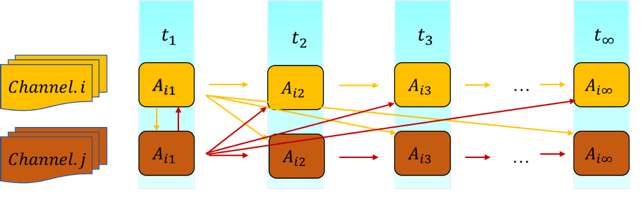
\includegraphics[width=0.8\textwidth]{2_ad_process}
\caption{广告在两个渠道上的生命周期}
\label{fig:2_ad_process}
\end{figure}

对于本渠道自身延迟的效果影响,我们可以使用强化学习中的累积折扣奖赏最大化处理;而对其他渠道产生的影响,我们通常要对全部的渠道进行建模,以捕捉到渠道之间的联系,但是,在广告投放的场景中,我们所能获得的数据非常少,如果使用仅有的少量数据对全部渠道进行建模,那么得到的模型自然时很差的。所以,一个自然的想法是,我们应该对每个渠道进行单独的建模,然后通过启发式的经验改进值函数的评估方法。

假设含有$n$个渠道的集合为$I=\{1,2,\cdots,n\}$,在某时刻,其他渠道$I\backslash\{i\}$对渠道$i$产生的影响记为$q_{i}^{'}$,定义为:
\begin{equation}\label{seq_ad_influence}
\begin{aligned}
q_{i}^{'}=\sum_{j\in I \backslash \{i\}} \sum_{k=0}^{\infty} \tau_{j,i,t+k+1} \cdot \gamma_{i}^{k} \cdot r_{j,t+k+1},\\
\tau_{j,i,t+k+1}=d \cdot \frac{c_{j,t+k+1}}{c_{i,t+k+1}},d<1.
\end{aligned}
\end{equation}

式$\eqref{seq_ad_influence}$中,$\gamma_{i}$表示渠道$i$的折扣因子,$\tau_{j,i,t+k+1}$是一个常数$d$乘以$t+k+1$时刻在第$j$个渠道上的花费与在第$i$个渠道上花费之比,$r_{j,t+k+1}$表示渠道$j$在$t+k+1$时刻所获的即时利润。从公式中可以看出,$\sum_{k=0}^{\infty} \gamma_{i}^{k} \cdot r_{j,t+k+1}$是近似为其他某一渠道获得的所获的累积利润,$\tau_{j,i,t+k+1}$通过某时刻第$j$个渠道上的花费与第$i$个渠道上花费的比值来反映渠道$j$对渠道$i$的投放效果的影响。

于是,考虑$q_{i}^{'}$并结合公式\eqref{seq2_qsa},可以得到改进的渠道$i$最优值函数的公式:
\begin{equation}
\label{seq_modified_q}
\begin{aligned}
q_{i}(S_{t},A_{t})&=\mathbb{E}[\sum_{k=0}^{\infty} \gamma_{i}^{k} r_{i,r+k+1} + \sum_{j \in I \backslash \{i\}} \sum_{k=0}^{\infty} \tau_{j,i,t+k+1} \cdot \gamma_{i}^{k} r_{j,t+k+1} | S_{t}=s, A_t = a]\\
&=\mathbb{E}[r_{i,t+1} + \gamma_{i} \sum_{k=0}^{\infty} \gamma_{i}^{k} r_{r+k+2} + \sum_{j \in \backslash \{i\}} \tau_{j,i,t+1}r_{j, t+1} \\
&+ \gamma_{i} \sum_{j \in \backslash \{i\}} \sum_{k=0}^{\infty} \tau_{j,i,t+k+2} \cdot \gamma_{i}^{k} r_{j,t+k+2} | S_{t}=s, A_t = a]\\
&=\mathbb{E}[r_{i,t+1} + \sum_{j \in I \backslash \{i\}} \tau_{j,i,t+1} r_{j, t+1} + \gamma_{i} q_{i}(S_{t+1},A_{t+1}) | S_{t}=s, A_t = a]\\
\end{aligned}
\end{equation}


因此,我们就可以将$t$时刻渠道$i$的Q值迭代的更新公式改为:
% \begin{equation}
% \begin{aligned}
\begin{dmath}
\label{seq_modified_Q}
Q_{i}(S_{t},A_{t})=Q_{i}(S_{t},A_{t})+\alpha_{i}(r_{i, t+1} + \sum_{j \in I \backslash \{i\}} \tau_{j,i,t+1} r_{j, t+1} + \gamma_{i} max_{a_{'}} Q_{i}(S_{t+1}, a^{'}) - Q_{i}(S_{t},A_{t}))
% \end{aligned}
% \end{equation}
\end{dmath}

\subsection{改进的探索方法}
在传统的Q-learning学习方法中,我们通常采用的ε-greedy的探索方法。其思想为:以概率$\epsilon$随机选择一个行为,以(1-$\epsilon$)的概率选择最优的策略。 $\epsilon-greedy$平衡了利用(exploitation)和探索(exploration),其中选取动作值函数最大的部分为利用,其他非最优动作仍有概率为探索部分。但是这种方法存在两个弱点:第一,它只关心从行为中得到了多少奖赏,而不知道它对该行为了解多少,即所有行为在任何时候都是平等的。所以,即使某一行为在初试经历中没有获得奖赏,它仍然有会被探索到。第二,因为采用随机抽样的方法,所以很容易被负面的经历所干扰。因此,特别是在小数据集的情况下,$\epsilon-greedy$的探索方法是不完全适用于广告投放的场景中。所以,我们在探索中,我们要不仅考虑到我们对该行为的了解程度,而且要减少随机采样的操作。所以,我们可以使用如下方式来选择行为:
\begin{equation}
\begin{aligned}
\argmax_{a}[Q(s,a)+\varphi \sqrt{\frac{ln n^{'}}{n_{a}^{'}}}]
\end{aligned}
\end{equation}
其中,$n^{'}$表示所有行为被选择的次数,$n_{a}^{'}$表示行为$a$被选择的次数,常数$\varphi > 0$控制了探索的程度。

因此,$t$时刻渠道$i$的Q值迭代的更新公式改为:

\begin{dmath}
\label{seq_modified_Q_}
Q_{i}(S_{t},A_{t})=Q_{i}(S_{t},A_{t})+\alpha_{i}(r_{i, t+1} + \sum_{j \in I \backslash \{i\}} \tau_{j,i,t+1} r_{j, t+1} + \gamma_{i} \max_{a_{'}} Q_{i}(S_{t+1}, \argmax_{a^{'}}[Q(S_{t},A_{t})+ \varphi_{i} \sqrt{\frac{ln n_{i}^{'}}{n^{'}_{i a^{'}}}}]) - Q_{i}(S_{t},A_{t}))
\end{dmath}



\subsection{批处理以及整体架构}
经过上述改进Q值函数的迭代公式以及探索方法后,对SVR+Q+MCKP分块模型的流程也要做相应的改进。因为在更新Q值函数时,需要考到到其他渠道的影响,这就要求我们应该利用同一时刻的投放数据同时对所有渠道进行更新。同时,为了使训练过程更加符合真是的投放场景,参考文献\citep{pednault2002sequential}采取了批强化学习的训练方法。改进后的模型伪代码如算法\eqref{algo:RBF-SVR+Q_final}和算法\eqref{algo:RBF-SVR+Q_2}所示。

\begin{algorithm}[htbp]
\small
\SetAlgoLined
\SetKwRepeat{Repeat}{repeat}{until} 
\SetKwData{Left}{left}\SetKwData{This}{this}\SetKwData{Up}{up}

输入:全部渠道的集合$I=\{1,2,\cdots,n\}$,$n$为渠道的总数;全部渠道的投放数据$O=\{O_{1},O_{2},\cdots,O_{n}\}$,其中$O_{i}=\{<\mathbf{s}_{i,t},c_{i,t},r_{i,t+1},\mathbf{s}_{i,t+1}>|t=1,\cdots,N_{i}\}$表示第$i$个渠道的数据集,$N_{i}$表示第$i$个渠道的数据量;Q函数的学习率$\alpha_{i}$,折扣因子$\gamma_{i}$,$i=1,2,\cdots,n$,最大迭代次数$P$,SVR+Q模型中的正则化参数$C$,RBF核函数的宽度$\sigma$\;

\For{$i=1$ \KwTo $n$}{
	利用算法$\ref{algo:DC}$求出渠道$i$的离散区间$\bm{\omega}_{i}=\{\omega_{i,1},\omega_{i,2},\cdots,\omega_{i,M_{i}+1}\}$,$M_{i}$表示第$i$个渠道形成的离散区间的个数\;
	将每个区间样本的平均花费值作为该区间所对应的行为值$a$,并且将此行为值添加到该区间的每个样本中,样本格式变为:$<\mathbf{s}_{i,t},c_{i,t},a_{i,t},r_{i,t+1},\mathbf{s}_{i,t+1}>$ \;
	按照行为值的不同,建立为$M_{i}$个样本单元$D_{i,h}$,$h=\{1,\cdots,M_{i}\}$,且此时,$D_{i,h}=\varnothing$ \;
}

数据转换:将全部渠道的数据$O$划分成$K$个情节$e$,即:$O=\{e_{k}|k=1,\cdots,K\}$,每个情节$e_{k}$包括$l_{k}$天的投放数据,即:$e_{k}=\{O^{'}_{j}|j=1,\cdots,l_{k}\}$,每一天的投放数据$O^{'}_{j}$又由$n$个渠道组成,即:$O^{'}_{j}=\{<\mathbf{s}_{k,j,i},c_{k,j,i},a_{k,j,i},r_{k,j+1,i},\mathbf{s}_{k,j+1,i}>|i=1,\cdots,n\}$\;

% 新增输入数据:SVR+Q模型中的正则化参数$C_{i,j}$,RBF核函数的宽度$\sigma_{i,j}$,,其中$i=1,2,\cdots,n$表示渠道号,$j=1,2,\cdots,M_{i}$表示渠道所对应的离散行为个数\;

\For{$k = 1$ \KwTo $K$}{
	\For{$j = 1$ \KwTo $l_{k}$}{
		\For{$i = 1$ \KwTo $n$}{
			按照算法\eqref{algo:RBF-SVR+Q_2}第10行的公式,计算样本的Q值,并将Q值添加到该样本中,其格式变为:$<\mathbf{s}_{k,j,i},c_{k,j,i},a_{k,j,i},r_{k,j+1,i},Q^{(0)}_{k,j,i}(\mathbf{s}_{k,j,i}),\mathbf{s}_{k,j+1,i}>$\;
			将该样本按照行为值分流到对应的样本单元中$D_{i,h}$,$h=\{1,\cdots,M_{i}\}$\;
		}
	}
}
$p=0$\;
\Repeat{$p=P$}{
	SVR+Q分块多路逼近迭代过程(算法$\ref{algo:RBF-SVR+Q_2}$)\;
	$p=p+1$ \;
}
输出各渠道的最终的Q值函数:$\text{Q}_{i}^{(P)}=\cup_{j=1,\cdots,l_{i}}\text{Q}_{i,j}^{(P)}$\; 
全渠道的Q值函数:$\text{Q}={\text{Q}_{i}^{(P)}}$,$i=1,\cdots,n$\;
$Res = MCKP(B,\text{Q})$\;
输出:最终的分配策略$Res$\;
\caption{SVR+Q+MCKP算法}
\label{algo:RBF-SVR+Q_final}
\end{algorithm}

\begin{algorithm}[htbp]
\small
\SetAlgoLined
\SetKwRepeat{Repeat}{repeat}{until} 
	\For{$i=1$ \KwTo $n$}{
		\For{$j=1$ \KwTo $M_{i}$}{
			对每个样本单元$D_{i,j}$,利用SVR+Q分块逼近模型进行回归建模,得到当前轮的Q值函数分块模型:$\text{Q}_{i,j}^{p}=f_{i,j}^{(p)}(\bm{s})=\sum_{m=1}^{N_{i,j}}(\hat{\alpha}_{i,j,m}^{(p)}-\alpha_{i,j,m}^{(p)})k(\bm{s},\bm{s}_{i,j,m})+b_{i,j}^{(p)}$,$N_{i,j}$表示第$i$个渠道的第$j$个样本空间中样本的个数\;
		}
	}

	\For{$k = 1$ \KwTo $K$}{
		\For{$j = 1$ \KwTo $l_{k}$}{
			\For{$i=1$ \KwTo $n$}{
				更新Q值函数:\\
				$\text{Q}_{k,j+1,i}^{(p+1)} = \text{Q}_{k,j+1,i}^{(p)} + \alpha_{i}^{(p)} (r_{k,j+1,i}+\gamma_{i} \argmax_{a^{'}}[f_{i,ID(a_{i}^{'})}^{(p)}(\bm{s}_{k,j+1,i})+\varphi_{i} \sqrt{\frac{ln n_{i}^{'}}{n_{i,ID(a_{i}^{'})}^{'}}}]) - \text{Q}_{k,j+1,i}^{(p)}$\;
				$ID(a_{i}^{'})$第$i$个渠道行为$a_{i}^{'}$所对应的编号,$n_{i}^{'}$ 为第$i$个渠道所有行为已经选择的次数,$n_{i,ID(a_{i}^{'})}^{'}$表示行为$ID(a_{i}^{'})$被选择的次数\;
				}
				利用上式更新在样本单元中的Q值\;
			}
		}

\caption{SVR+Q分块逼近的迭代过程}
\label{algo:RBF-SVR+Q_2}
\end{algorithm}


\section{本章小结}
在本章中,首先分析了在直复营销体系下,基于广告代理商的投放预算分配问题,并说明了将全渠道的LTV作为评价广告投放效果的指标,以此作为选择强化学习解决该问题的出发点。另外,又分析在应用时所面临的场景复杂、数据量少以及预算约束等问题。然后,在小数据集下,针对值函数逼近问题提出了SVR+Q多路逼近模型,加快收敛速度的同时提高手链精度,并将SVR+Q与MCKP结合,应用于多渠道资金分配问题。最后,提出一个花费空间离散化的方法,以更好的应用SVR+Q+MCKP模型、针对多渠道之间的影响提出一种改进值函数的估计方法,而且提出了一个在小数据集下高效的探索方法。


